\section{Evidencia empírica}

La ontología propuesta se sustenta en tres conjuntos de validaciones realizadas con el mismo pipeline RECD+RQA Config B.

\subsection{Regímenes caóticos y cercanos al punto de Feigenbaum}

En el mapa logístico acoplado de cuatro componentes con $r=3.8$ y acoplamiento base 0.02, sometido a dos inyecciones de acoplamiento en $t=380$ y $t=920$, el detector identificó 121 picos hiperestructurales. El adelanto medio a las inyecciones ground-truth fue sustancial y estadísticamente superior al obtenido con picos aleatorios de igual cardinalidad.

En contraste, cuando el sistema opera cerca del punto de acumulación de Feigenbaum ($r \approx 3.56995$), el detector se vuelve extremadamente conservador. Con inyecciones moderadas de acoplamiento, se obtuvieron cero picos estructurales. La hiper-persistencia ya constituye el régimen basal, de modo que las intensificaciones relativas resultan indistinguibles.

El atractor de Lorenz (tres variables $x,y,z$, parámetros clásicos, $T=5000$, $dt=0.02$) con inyecciones de $\rho$ en $t=1500$ y $t=3200$ produjo 123 picos hiperestructurales, situándose en un comportamiento intermedio.

\subsection{Rol de la antisincronización}

El análisis explícito de la serie temporal de antisincronización $A(k)$ reveló un patrón consistente y estadísticamente significativo: los picos hiperestructurales tienden a ocurrir cuando la antisincronización \textit{disminuye}.

En el mapa logístico $r=3.8$, la media de antisincronización en ventanas de $\pm 50$ pasos alrededor de los picos estructurales fue significativamente inferior a la media del resto de la serie (prueba de Mann-Whitney $p=0.0229$). El mismo patrón, aunque de menor magnitud, se observó en el atractor de Lorenz. Además, los valores de antisincronización en los 100 pasos previos a cada pico fueron aún más bajos, sugiriendo que la alineación de escalas de persistencia precede a la emergencia del pico hiperestructural.

\begin{importantbox}
La intensificación local del presente (Capa 1) genera efectos estructurales (Capa 3) con mayor probabilidad cuando los módulos presentan escalas de persistencia más coherentes entre sí (baja antisincronización, Capa 2). De lo contrario, la intensificación permanece como un fragmento aislado que el sistema puede absorber sin reorganizarse. (Este efecto de filtrado probabilístico ascendente se conoce ocasionalmente, con valor heurístico secundario, como «resistencia ascendente».)
\end{importantbox}

\begin{figure}[htbp]
\centering
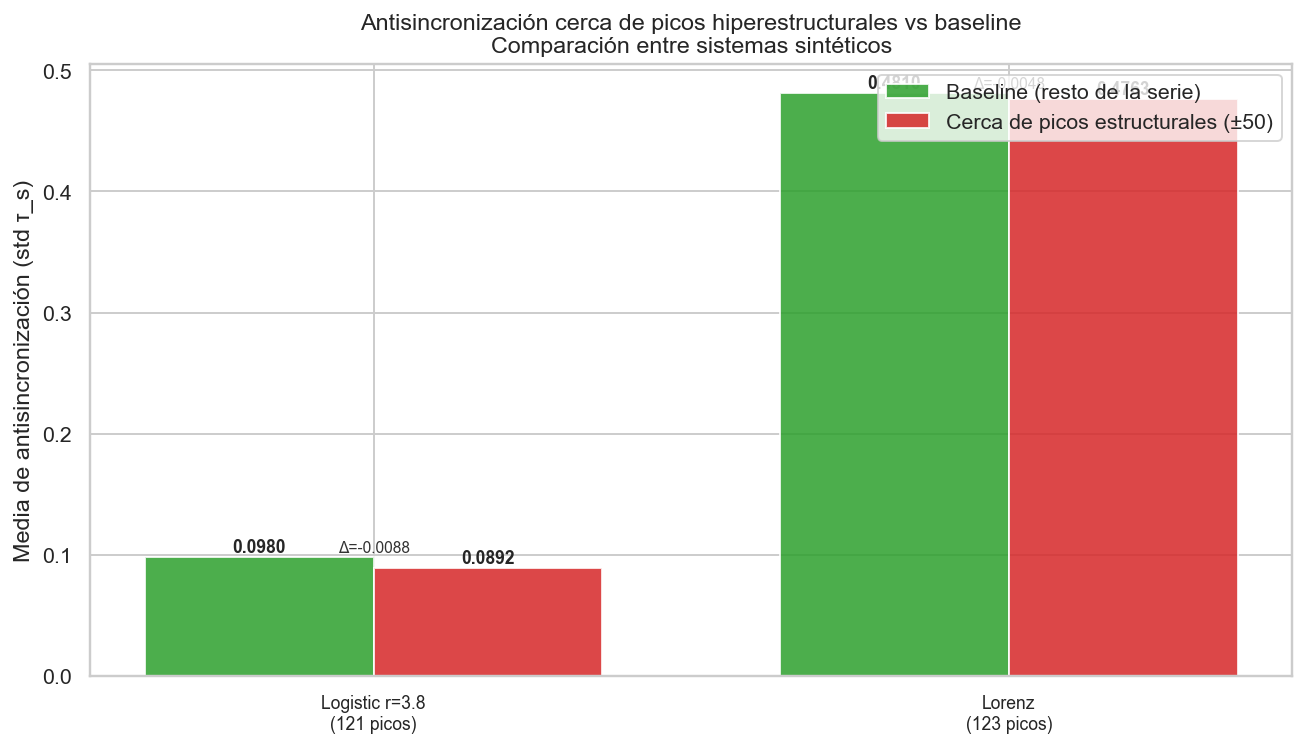
\includegraphics[width=0.9\linewidth]{figures/fig_antisincronizacion_comparativa.png}
\caption{Comparación de la antisincronización (desviación estándar de $\tau_s$) cerca de picos hiperestructurales versus el baseline (resto de la serie) en los dos sistemas sintéticos principales. En ambos casos se observa una reducción sistemática de la antisincronización en las proximidades de los picos (121 en el mapa logístico $r=3.8$; 123 en el atractor de Lorenz). Esta evidencia empírica apoya directamente que la transición de la Capa 1 (presente local intensificado) a la Capa 3 (reorganización estructural) se ve favorecida por una disminución de la fragmentación (Capa 2).}
\label{fig:antisinc_comparativa}
\end{figure}

\begin{figure}[htbp]
\centering
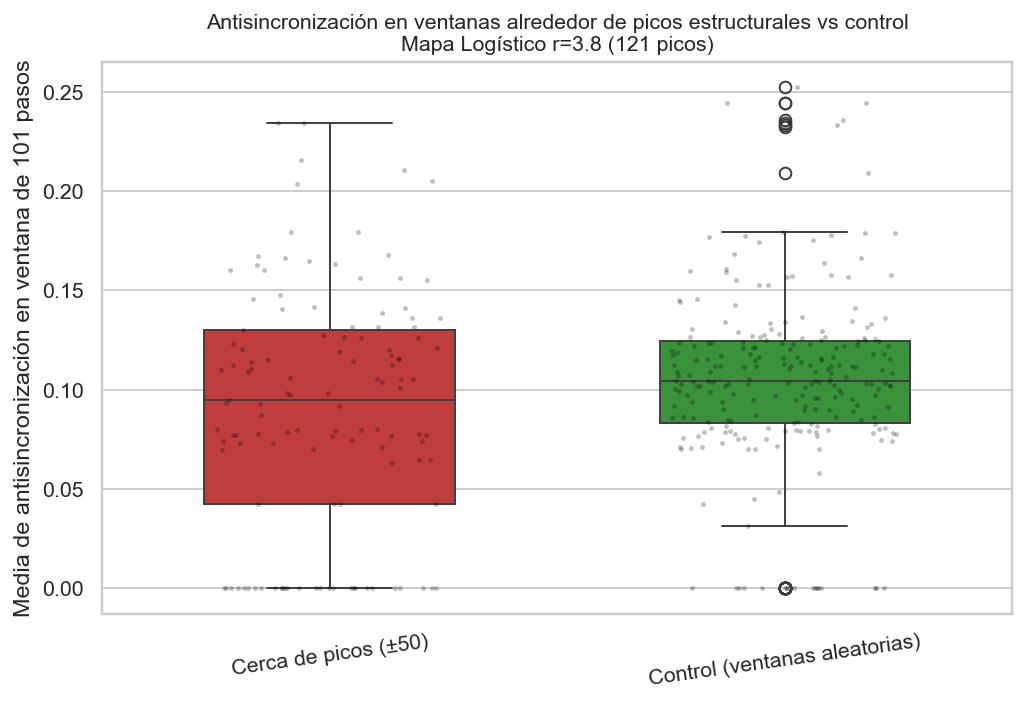
\includegraphics[width=0.8\linewidth]{figures/fig_antisinc_logistic_box.png}
\caption{Distribución de la media de antisincronización en ventanas de $\pm 50$ pasos alrededor de picos estructurales frente a ventanas de control aleatorias (mapa logístico $r=3.8$). La diferencia es estadísticamente significativa (Mann-Whitney $p=0.0229$), confirmando que los picos hiperestructurales ocurren preferentemente en contextos de mayor coherencia entre componentes.}
\label{fig:antisinc_box}
\end{figure}

\subsection{Robustez al ruido}

Cuando se añadió ruido gaussiano controlado (0 \%, 5 \%, 10 \% y 15 \% de la desviación estándar de cada componente) al mapa logístico $r=3.8$, el número de picos estructurales descendió de 121 a 100, mientras que los cambios por norma de Frobenius permanecieron esencialmente invariantes. El detector conserva utilidad práctica hasta ~10--15 \% de ruido, con degradación gradual. Esto indica que la intensificación del presente posee estabilidad estructural que trasciende fluctuaciones superficiales.

\begin{figure}[htbp]
\centering
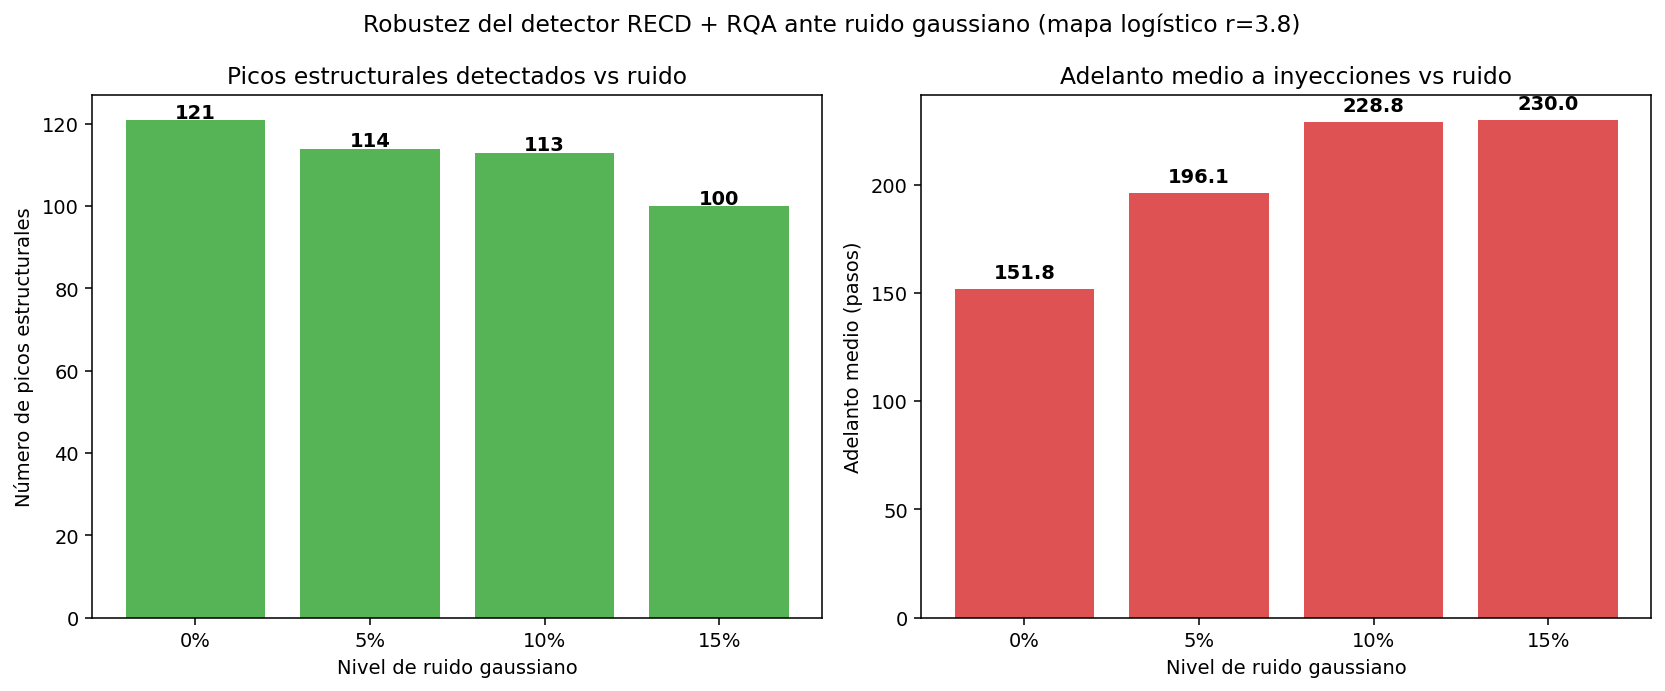
\includegraphics[width=0.9\linewidth]{figures/fig_ruido_robustez_metricas.png}
\caption{Robustez del detector de picos hiperestructurales (RECD + RQA Config B + hiper-persistencia) ante ruido gaussiano aditivo en el mapa logístico acoplado $r=3.8$. El número de picos estructurales detectados (izquierda) y el adelanto medio a las inyecciones conocidas (derecha) se mantienen razonablemente estables hasta niveles de ruido del 10--15\%. La invariancia del número de cambios estructurales por norma de Frobenius sugiere que la estructura subyacente de coherencias persiste más allá de las fluctuaciones superficiales, apoyando la idea de que la intensificación del presente (Capa 1) tiene un sustrato estructural que no se reduce a ruido.}
\label{fig:ruido_robustez}
\end{figure}

\subsection{Implicaciones para la ontología}

Los hallazgos empíricos constituyen evidencia de que la \textit{discreción} detectada por el RECD corresponde a transiciones entre distintos niveles de integración de la persistencia. La universalidad de Feigenbaum, la robustez al ruido y —de manera especialmente relevante— el papel regulador de la antisincronización (reducción sistemática y estadísticamente significativa previa a picos estructurales) convergen en la estructura jerárquica que sigue. Esta evidencia —la aparición preferente de picos hiperestructurales en contextos de baja antisincronización, su adelanto estadísticamente significativo respecto a las inyecciones, y la conservación de la capacidad detectiva ante ruido moderado— motiva directamente tanto la partición ontológica en tres capas como la caracterización del filtrado probabilístico bidireccional como el mecanismo estructural que regula la probabilidad de que una intensificación local (Capa 1) logre producir reorganización global (Capa 3). Las secciones siguientes articulan esta transición.